\section{Reti Posti e Transizioni}

Le reti Posti e Transizioni sono un'estensione delle reti di Petri, in cui le condizioni, invece di essere solo vere o false, hanno una capacità $K$ (queste condizioni sono chiamate \textbf{pposti}).
A questo punto, l'evento può richiedere una certa capacità per poter scattare (lo scatto si chiamac\textbf{transizione}).
\\
\\
In particolare, $\Sigma = (S, T, F, K, W, M_0)$ è un \textbf{sistema Posti e Transizioni} (P/T) se e solo se

\begin{itemize}
	\item $(S, T, F)$ è una rete
	\item $K : S \to \mathbb N^+ \cup \{ \infty \}$ è la funzione \textbf{capacità dei posti}

	\item $W : F \to \mathbb N$ è la funzione \textbf{peso degli archi}

	\item $M_0 : S \to \mathbb N : \forall s \in S, \quad M_0(s) \leq K(s)$ è la \textbf{marcatura iniziale}
\end{itemize}

\subsection{Regola di transizione}

Sia $t \in T$ e $M : S \to \mathbb N$ una marcatura, allora abbiamo che $M[t>$ se e solo se
\[
	\forall s \in S, \quad
	M(s) \geq W(s, t) \quad \wedge \quad M(s) + W(t, s) \leq K(s)
\]
inoltre, $M[t>M'$ se e solo se
\[
	M[t>
	\quad \wedge \quad
	\forall s \in S,
	\quad
	M'(s) = M(s) - W(s, t) + W(t, s)
\]

\subsection{Marcature raggiungibili}

Sia $\Sigma = (S, T, F, K, W, M_0)$ un sistema P/T, l'insieme delle \textbf{marcature raggiungibili} di $\Sigma$, denotato $[M_0>$, è il più piccolo insieme tale che
\begin{itemize}
	\item $M_0 \in [M_0>$
	\item se $M \in [M_0> \wedge \ \exists t \in T : M[t>M'$ allora $M' \in [M_0>$
\end{itemize}

\subsection{Multiset abilitato}
Sia $\Sigma = (S, T, F, K, W, M_0)$ un sistema P/T,
\begin{itemize}
	\item Un \textbf{multiset} $U : T \to \mathbb N$ è \textbf{concorrentemente abilitato} in $M \in [M_0>$ ($U$ è un \textbf{passo} $M[U>$) se e solo se
	      \[
		      \forall s \in S,
		      \quad
		      \sum_{t \in T}{U(t) \cdot W(s, t)} \leq M(s)
		      \quad \wedge \quad
		      M(s) + \sum_{t \in T}{U(t) \cdot W(t, s) \leq K(s)}
	      \]
	\item Un \textbf{multiset} $U$ abilitato in $M$ può \textbf{occorrere} generando $M'$, $M[U>M'$, se e solo se
	      \[
		      \forall s \in S,
		      \quad
		      M'(s)
		      =
		      M(s)
		      -
		      \sum_{t \in T}{U(t) \cdot W(s, t)}
		      +
		      \sum{t \in T}{U(t) \cdot W(t, s)}
	      \]
	\item $U_\Sigma$ è l'\textbf{insieme dei passi} di $\Sigma$
	      \[
		      U_\Sigma
		      =
		      \{
		      U : T \to \mathbb N \ | \ \exists M, M' \in [M_0> \ : M[U > M'
		      \}
	      \]
\end{itemize}

\subsection{Grafo di Raggiungibilità}
Sia $\Sigma = (S, T, F, K, W, M_0)$ un sistema P/T. $RG(\Sigma) = ([M_0>, U_\Sigma, A, M_0)$ è il \textbf{grafo di raggiungibilità} di $\Sigma$, dove
\[
	A
	=
	\{
	(M, U, M') : M, M' \in [M_0> \ \wedge \ U \in U_\Sigma \ \wedge \ M[U>M'
	\}
\]
Se U è una singola transizione si ha il \textbf{grafo di raggiungibilità sequenziale} $SRG(\Sigma)$
\\
\\
\textbf{Attenzione}: in generale, la diamond property \textbf{non} è più valida! Questo a causa dei self-loop.

\subsection{Contatto e Complementazione}

$t$ è una situazione di \textbf{contatto} in $M$ se e solo se
\[
	\forall s \in S,
	\
	W(s, t) \leq M(s)
	\quad \wedge \quad
	\exists s \in S : M(s) + W(t, s) > K(s)
\]
Come nei sistemi elementari, anche nelle reti Posti e Transizioni è \textbf{sempre} possibile aggiungere posti per \textbf{eliminare} le situazioni di contatto senza alterare il comportamento del sistema.
\\
\\
Sia $\Sigma = (S, T, F, K, W, M_0)$ un sistema P/T con capacità (tale che per alcuni posti la capacità sia finita), allora si \textbf{complementano i posti a capacità finita} ottenendo il sistema P/T $\Sigma' = (S', T, F', K', W', M_0')$ tale che
\begin{itemize}
	\item $S'= S \cup S_1$, dove $S_1 = \{ \bar s \ | \ s \in S \ \wedge \ K(s) < \infty \}$
	\item $F'= F \cup F_1$, dove
	      \[
		      F_1 = \{ (\bar s, t) \ | \ (t, s) \in F \ \wedge \ K(s) < \infty\} \cup \{ (t, \bar s) \ | \ (s, t) \in F \ \wedge \ K(s) < \infty \}
	      \]
	\item $\forall s' \in S', \ K'(s') = \infty$
	\item $W'(\bar s, t) = W(t, s)$ e $W'(t, \bar s) = W(s, t), \ \forall t \in T, \forall \bar s \in S_1$\\
	      $W'(s, t) = W(s, t)$ e $W'(t, s) = W(t, s), \ \forall t \in T, \forall s \in S$
	\item $M'_0(s) = M_0(s), \ \forall s \in S$\\
	      $M'_0(\bar s) = K(s) - M_0(s), \ \forall \bar s \in S_1$
\end{itemize}

\noindent
$\Sigma'$ è senza vincoli di capacità e quindi si può dimostrare che $\Sigma'$ è \textbf{senza contatti} e che il suo grafo di raggiungibilità $RG(\Sigma')$ è \textbf{isomorfo} a $RG(\Sigma)$. Inoltre, per ogni marcatura raggiungibile $M'$ in $\Sigma'$, vale: $\forall \bar s \in S_1, \ M'(s) + M'(\bar s)= K(s)$
\\
\\
Un sistema P/T $\Sigma = (S, T, F, K, W, M_0)$ è \textbf{senza contatti} se e solo se
\[
	\forall M \in [M_0>, \ \forall t \in T, \forall s \in S
	\quad
	M(s) \geq W(s, t) \implies M(s) + W(t, s) \leq K(s)
\]

Se $\Sigma = (S, T, F, K, W, M_0)$ è un sistema P/T \textbf{senza contatti}, allora $t$ è \textbf{abilitata} in $M \in [M_0>$ (cioè $M[t>$) se e solo se
\[
	\forall s \in S, \quad M(s) \geq W(s, t)
\]
\subsection{Reti marcate}
Un sistema P/T $\Sigma = (S, T, F, K, W, M_0)$ è una \textbf{rete marcata} se e solo se
\[
	\forall s \in S, \ M_0(s) \in \mathbb N
	\ \wedge \ K(s) = \infty \quad \wedge \quad
	\forall t \in T, \ W(s, t) \leq 1 \ \wedge \
	W(t, s) \leq 1
\]
Ovvero i Posti hanno capacità illimitata e gli archi hanno tutti peso 1. Le reti marcate sono denotate $(S, T, F, M_0)$ in quanto $K$ e $W$ sono ridondanti.
\\
\\
Una rete marcata è \textbf{sicura} (\textbf{safe}) se e solo se
\[
	\forall M \in [M_0>, \ \forall s \in S, \quad M(s) \leq 1
\]
\textbf{Nota}: in una rete marcata i loop possono essere abilitati.

\subsection{Matrici Backward e Forward}
Sia $\Sigma = (S, T, F, K W, M_0)$ un sistema P/T tale che $\forall s \in S, \ K(s) = \infty$. Allora $\Sigma$ può essere rappresentato da 2 matrici con $|S|$ righe e $|T|$ colonne:

\begin{itemize}
	\item $\underline B : S \times T \to \mathbb N$ matrice \textbf{backward}, con $\underline B_{i,j} = W(s_i, t_j)$
	\item $\underline F : S \times T \to \mathbb N$ matrice \textbf{forward}, con $\underline F_{i, j} = W(t_j, s_i)$
\end{itemize}
La marcatura $M_0$ può essere rappresentata da un vettore colonna $\underline M_0$ di $|S|$ elementi.
\\
\\
\textbf{Esempio:}
\begin{multicols}{2}
	\begin{center}
		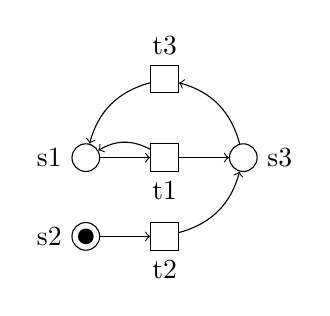
\begin{tikzpicture}
			\node[shape = circle, draw, minimum size=1em, label=left:s1] (s1) at (-1, 0){};
			\node[shape = circle, draw, minimum size=1em, label=left:s2] (s2) at (-1, -1){};
			\node[shape = circle, draw, minimum size=1em, label=right:s3] (s3) at (1, 0){};


			\fill (s2) circle (1mm);

			\node[shape=rectangle, draw,  minimum size=1em, label=below:t1] (t1) at (0, 0){};
			\node[shape=rectangle, draw,  minimum size=1em, label=below:t2] (t2) at (0, -1){};
			\node[shape=rectangle, draw,  minimum size=1em, label=above:t3] (t3) at (0, 1){};


			\draw[->] (s2) to (t2);
			\draw[->, bend right] (t2) to (s3);
			\draw[->, bend right] (s3) to (t3);
			\draw[->, bend right] (t3) to (s1);
			\draw[->] (s1) to (t1);
			\draw[->, bend right] (t1) to (s1);
			\draw[->] (t1) to (s3);
		\end{tikzpicture}
	\end{center}
	\columnbreak
	\begin{center}
		\begin{tabular}{|c|c|c|c|}
			\hline
			\textbf{B} & t1 & t2 & t3 \\ \hline
			s1         & 1  &    &    \\ \hline
			s2         &    & 1  &    \\ \hline
			s3         &    &    & 1  \\ \hline
		\end{tabular}
		\hspace{1em}
		\begin{tabular}{|c|c|c|c|}
			\hline
			\textbf{F} & t1 & t2 & t3 \\ \hline
			s1         & 1  &    & 1  \\ \hline
			s2         &    &    &    \\ \hline
			s3         & 1  & 2  &    \\ \hline
		\end{tabular}
		\\
		\vspace{1em}
		\begin{tabular}{|c|}
			\hline
			\textbf{$\mathbf{M_0}$} \\ \hline
			\                       \\ \hline
			1                       \\ \hline
			2                       \\ \hline
		\end{tabular}

	\end{center}
\end{multicols}

\subsection{Regola di Scatto}

Sia $M : S \to \mathbb N$ una marcatura e $t \in T$, allora

\[
	M[t> \quad \iff \quad \forall s \in S, \ M(s) \geq W(s, t) \quad \iff \quad \underline M \geq \underline B(t)
\]
\vspace{1em}
\[
	\begin{aligned}
		M[t>M'
		\quad & \iff \quad
		M[t> \ \wedge \ \ \forall s \in S, \ M'(s) = M(s) - W(s, t) + W(t, s)
		\\
		      & \iff \quad
		M[t> \ \wedge \ \ \bf{\underline M' = \underline M - \underline B(t) + \underline F(t)}
	\end{aligned}
\]
\\
\\
\textbf{Esempio nel caso precedente:}
\[
	M_0[t_2>M
\]
\vspace{1em}
\begin{center}
	\begin{tabular}{|c|}
		\hline
		\textbf{$\mathbf{M}$} \\ \hline
		\                       \\ \hline
		\                       \\ \hline
		4                       \\ \hline
	\end{tabular}
	=
	\begin{tabular}{|c|}
		\hline
		$\mathbf{M_0}$ \\ \hline
		\                       \\ \hline
		1                       \\ \hline
		2                       \\ \hline
	\end{tabular}
    $-$
	\begin{tabular}{|c|}
		\hline
        $\mathbf{B_{t2}}$ \\ \hline
		\                       \\ \hline
		1                       \\ \hline
		\                       \\ \hline
	\end{tabular}
	+
    \begin{tabular}{|c|}
		\hline
        $\mathbf{F_{t2}}$ \\ \hline
		\                       \\ \hline
		\                       \\ \hline
		2                       \\ \hline
	\end{tabular}
\end{center}

\subsection{Matrice di Incidenza}
Sia $\Sigma = (S, T, F, K, W, M_0)$ un sistema P/T tale che $\forall s \in S, \ K(s) = \infty$ e sia \textbf{senza cappi}. Allora il sistema può essere rappresentato da un'unica matrice $\underline N : S \times T \to \mathbb N$.
\\
\\
La matrice $\underline N$ con $|S|$ righe e $|T|$ colonne è la \textbf{matrice di incidenza} di $N = (S, T, F, K, W)$ se e solo se 
\[
    \underline N(i, j) = W(t_j, s_i) - W(s_i, t_j)
\]
\[
    \implies \underline N = \underline F - \underline B
\]

\subsection{Equazione di Stato (Firing Lemma)}

Sia $\sigma \in T^*$ una sequenza di transizioni. 
Il \textbf{vettore di Parikh} di $\sigma$ è il vettore $\underline{c_\sigma}$ di $|T|$ elementi tale che $\underline{c_\sigma}(t_i)$ è il numero di occorrenze di $t_i$ in $\sigma$.

Abbiamo quindi che
\[
    M_0[\sigma>M_1
    \implies
    \underline{M_0} + \underline N \cdot \underline{c_\sigma}  =  \underline{M_1}
\]

Quest'ultima è detta \textbf{equazione di stato}. La validità dell'equazione di stato è \textbf{condizione necessaria ma non sufficiente} affinchè una sequenza di transizioni generi una marcatura in un sistema.

\subsection{Vettore Realizzabile}

Un vettore $\underline c \in \mathbb N^T$ è \textbf{realizzabile} da una marcatura $M$ se c'è una sequenza di transizioni $\sigma$ tale che $M[\sigma >$, con $\underline c = \underline{c_\sigma}$ vettore di Parikh di $\sigma$.

\textbf{slide lez 6}
